\documentclass[manuscript,review,anonymous]{acmart}

%% ------------------------------------------------------------------
%% BASiS 日本語版ドラフト（英語版の内容確認用）
%% pdfLaTeX + CJKutf8 でコンパイルする日本語確認版です．
%% コンパイル順: pdflatex -> bibtex -> pdflatex -> pdflatex
%% ------------------------------------------------------------------

\usepackage{amsmath}
\usepackage{booktabs}
\usepackage{graphicx}
\usepackage{tabularx}
\usepackage{array}
\usepackage{comment}
\usepackage{pifont}

%% Japanese support compatible with pdfLaTeX/Overleaf free-plan builds.
%% CJKutf8 uses TeX Live's bundled Japanese fonts, so no system-font search is needed.
\usepackage{CJKutf8}
\usepackage{CJKspace}

%% Load the bundled Mincho font definition early so acmart's bold/italic
%% requests can be mapped to shapes available under pdfLaTeX.
\makeatletter
\input{c70min.fd}
\makeatother
\DeclareFontShape{C70}{min}{b}{n}{<->ssub*min/bx/n}{}
\DeclareFontShape{C70}{min}{m}{it}{<->ssub*min/m/n}{}
\DeclareFontShape{C70}{min}{b}{it}{<->ssub*min/bx/n}{}

%% Activate CJK decoding for the whole document without opening a nested
%% environment. This keeps acmart's title/keyword metadata assignments global
%% and also keeps CJK active while deferred floats and end-document hooks run.
\makeatletter
\newcommand{\ActivateCJKForPDFLaTeX}{%
  \CJKnospace
  \CJK@envStart{}{UTF8}{min}%
}
\makeatother

\setcopyright{acmlicensed}
\acmConference[IUI '27]{32nd Annual ACM Conference on Intelligent User Interfaces}{February 8--11, 2027}{Helsinki, Finland}
\acmDOI{}
\acmISBN{}

\begin{document}
\ActivateCJKForPDFLaTeX

\title{BASiS:ベイズ的データ選別による目的特化対話システムの会話行動適応}

\author{Anonymous Author(s)}
\affiliation{%
  \institution{Institution withheld for review}
  \city{City}
  \country{Country}
}
\renewcommand{\shortauthors}{Anonymous Author(s)}

\begin{abstract}
本論文では，小規模高品質な対話コーパスを単なる発話例の集合として利用するのではなく，そこに暗黙に含まれる対話の進め方を，会話状態の遷移と各状態における応答戦略の確率分布としてモデル化し，このモデルを大規模汎用コーパスから学習データを選ぶ基準へ転用する手法BASiS（Bayesian Style-based Selection）を提案する．本研究は，相手の状態や対話局面に応じて対話を進行させる必要がある場面に着目する．こうした対話の質を支えるのは，個々の発話内容だけではなく，相手の状況をどのように捉え，どのタイミングでどの対話方策を用いるかという、インタラクションにおける手続き的知識である．しかし，このような知識は小規模な高品質対話コーパスに暗黙的に含まれている一方，そのままでは大規模なLLM学習に十分なデータ量を確保できない．BASiSは，この知識を会話状態・応答戦略・状態遷移の確率モデルとして抽出し，大規模汎用コーパスの学習データ選別基準へ変換することで，少量の高品質対話に含まれる知識を大規模学習へスケールさせる．
BASiSでは，小規模コーパスから会話状態，応答戦略，状態遷移を抽出し，それらをベイズ的対話モデルとして表現する．次に，大規模コーパスに含まれる対話を，目的の会話スタイルへの適合度に基づいてスコアリングし，学習データを選別する．さらに，選別したデータから選好ペアを構築し，Direct Preference Optimization（DPO）を用いてLLMを学習する．これにより，詳細な対話ガイドラインを人手で設計する負担を軽減しながら，一般的な品質や話題の類似性だけでは捉えにくい応答のタイミングや複数ターンにわたる対話の進行を，データ選別に反映できる．また，単一の応答戦略に固定するのではなく，会話状態を確率分布として保持することで，同一の文脈に対する複数の妥当な応答戦略を維持できる．
感情支援，数学チュータリング，医療問診を対象として，学習前のベースモデル，BASiSによる選別データで学習したモデル，および目的コーパスのカテゴリ内から無作為に選別したデータで学習したモデルを比較することで，BASiSを評価した．その結果，BASiSは三領域の全21評価軸で最高の平均値を示し，感情支援と数学チュータリングでは広範な有意改善が確認された．
\end{abstract}

\begin{CCSXML}
<ccs2012>
 <concept>
  <concept_id>10010147.10010178.10010179</concept_id>
  <concept_desc>Computing methodologies~Natural language generation</concept_desc>
  <concept_significance>500</concept_significance>
 </concept>
 <concept>
  <concept_id>10010147.10010178.10010179.10010182</concept_id>
  <concept_desc>Computing methodologies~Discourse, dialogue and pragmatics</concept_desc>
  <concept_significance>500</concept_significance>
 </concept>
 <concept>
  <concept_id>10003120.10003121.10003122.10003334</concept_id>
  <concept_desc>Human-centered computing~Natural language interfaces</concept_desc>
  <concept_significance>300</concept_significance>
 </concept>
 <concept>
  <concept_id>10010147.10010257.10010293.10010294</concept_id>
  <concept_desc>Computing methodologies~Learning from implicit feedback</concept_desc>
  <concept_significance>100</concept_significance>
 </concept>
</ccs2012>
\end{CCSXML}

\ccsdesc[500]{Computing methodologies~Natural language generation}
\ccsdesc[500]{Computing methodologies~Discourse, dialogue and pragmatics}
\ccsdesc[300]{Human-centered computing~Natural language interfaces}
\ccsdesc[100]{Computing methodologies~Learning from implicit feedback}

\keywords{目的特化対話システム, 会話スタイル, データ選別, ベイズ的対話モデリング, 選好最適化, 感情支援対話, 大規模言語モデル}

\maketitle

%% Keep PDF metadata ASCII-only. acmart writes metadata again at end of the
%% document, after the CJK environment has closed; Japanese metadata would
%% otherwise trigger a pdfLaTeX Unicode error at \end{document}.
\hypersetup{
  pdftitle={BASiS: Japanese Content-Review Draft},
  pdfauthor={Anonymous Author(s)},
  pdfsubject={Purpose-specific dialogue style adaptation},
  pdfkeywords={dialogue systems, conversational style, data selection, Bayesian modeling, DPO}
}

\section{はじめに}
\label{sec:intro}

Instruction tuningやRLHFの発展により，近年の大規模言語モデル（LLM）は，指示に従って正確な応答を生成し，多様な話題について自然で一貫した複数ターン対話を行えるようになった\cite{ouyang2022instructgpt}．一方，感情支援，数学チュータリング，医療問診などの目的特化対話では，正しい情報を提示するだけでなく，相手の状態や対話の段階に応じて適切な応答方針を選ぶ必要がある\cite{rashkin2019empathetic,liu2021esconv}．例えば，相手の感情を受け止めてから助言へ移ること，学習者自身の推論を促すこと，必要な症状を適切な順序で聞き出すことが求められる．このような会話スタイルは，目的に沿って構築された小規模高品質コーパスに表れているが，そのままLLMの学習に用いるにはデータ量が限られる．これに対し，大規模汎用コーパスはデータ量と多様性に優れるものの，目的の会話スタイルに適合する対話を十分に含むとは限らない．そこで，小規模高品質コーパスに含まれる対話の進め方を，LLMの実際の応答生成へ反映する方法が必要となる．

目的特化対話に適した応答を生成するため，既存研究では複数のアプローチが検討されている．ガイドラインに基づく応答制御では，望ましい対話方針をあらかじめ明示的に定義し，その方針に従うように応答生成を制御する．WenらのGuidedTODは，タスク指向対話の流れを確率的に表現し，対話の進行に応じてガイドラインに基づく方針を更新しながら応答候補を再ランキングすることで，既存手法よりも高いガイドライン遵守性能を示した\cite{wen2025guidedtod}．また，対話履歴から次の対話行動や応答戦略を予測する研究も行われている．Ganeshらは，授業対話において教師が次に取るtalk moveを予測し\cite{ganesh2021teacher}，WanらのEmoDynamiXは，ユーザの複数の感情状態と応答戦略の関係を異種グラフとしてモデル化した\cite{wan2025emodynamix}．Rudolphらは，カウンセリング対話から得た遷移行列を次対話行為予測の正則化に用いた\cite{rudolph2026transition}．さらに，LLMの学習に用いるデータの選別に関する研究では，少量であっても高品質なデータを適切に選ぶことで，効率的にモデルの振る舞いを調整できることが示されている\cite{zhou2023lima,zhang2025datasurvey}．

しかし，これらの既存研究には二つの課題がある．第一に，ガイドラインに基づく応答制御では，目的や領域ごとに望ましい対話方針を人手で記述する必要がある．会話のトーン，応答のタイミング，複数ターンにわたる対話の進め方など，コーパスに暗黙的に表れる会話スタイルを網羅的なルールとして明示することは難しい．第二に，対話行動や応答戦略に関する既存研究は，対話の流れをモデル化して次の行動や戦略を予測することを主な対象としており，その予測に基づく自然言語応答の生成や，生成応答の品質評価までは扱っていない．そのため，コーパスから学習した対話構造を，実際の応答生成へどのように反映するかは十分に検討されていない．

これらの課題を解決するため，本研究では，小規模高品質コーパスに基づくベイズ的データ選別を通じて，目的特化対話に求められる会話スタイルをローカルLLMへ反映する手法「BASiS（Bayesian Style-based Selection）」を提案する．BASiSでは，まずLLMを用いて小規模高品質コーパスを分析し，各対話を，会話相手の状況や対話段階を表す会話状態，共感・質問・助言などの応答方針を表す応答戦略，および応答によって生じる状態遷移として構造化する．次に，抽出した会話構造から，状態間の遷移確率と各状態における応答戦略の観測尤度を持つベイズ的対話モデルを構築する．構築したモデルを用いて，大規模汎用コーパスに含まれる各対話データを目的の会話スタイルへの適合度に基づいてスコアリングし，学習に用いるデータを選別する．最後に，選別したデータから選好ペアを構築し，LoRAを適用したDirect Preference Optimization（DPO）によってローカルLLMを学習することで，小規模コーパスに含まれる会話スタイルをモデルに反映する．

BASiSの特徴は，小規模コーパスに含まれる会話スタイルを，個別の応答表現や人手で作成した詳細なガイドラインとしてではなく，会話状態と応答戦略の確率的な遷移として表現する点にある．これにより，目的ごとの詳細な対話ガイドラインの手動記述を前提とせず，コーパスに暗黙的に含まれる対話の流れをデータ選別に利用できる．また，対話状態を確率分布として保持し，候補応答から得た観測によってベイズ更新することで，現在の会話履歴と応答後の状態遷移を選別基準に反映する．さらに，参照する小規模コーパスと選別対象となる大規模コーパスを変更することで，感情支援，数学チュータリング，医療問診など，異なる目的特化対話に同じ手順を適用できる．選別したデータをLoRAベースのDPO学習に用いることで，ローカルLLMの一般的な対話能力を活用しながら，目的の会話スタイルを反映する．

本論文の構成は以下の通りである．第\ref{sec:relwork}章では，ガイドラインに基づく応答制御，対話履歴に基づく対話行動・応答戦略予測，およびLLMの学習データ選別に関する関連研究を紹介する．第\ref{sec:method}章では，提案手法BASiSの学習パイプラインと各モジュールの機能を述べる．第\ref{sec:evaluation}章では，BASiSの有効性を検証する実験，実験結果，および考察について述べる．最後に，第\ref{sec:conclusion}章で本研究をまとめる．


\section{関連研究}
\label{sec:relwork}

目的に応じた対話システムの振る舞いを実現する方法として，望ましい応答方針を自然言語のガイドラインとして与え，応答生成を制御する研究が行われている．Guptaらは，ガイドラインが適用される会話文脈と，応答に含めるべき内容を自然言語で記述するDialGuideを提案した\cite{gupta2023dialguide}．DialGuideでは，ガイドラインの選択，ガイドラインに基づく応答生成，および生成応答がガイドラインを満たすかの検証を扱い，日常対話と安全性に関する対話データを用いた実験により，開発者のガイドラインに従った安全かつ対話性の高い応答を生成できることが示された．Wenらは，タスク指向対話における一連のガイドラインをマルコフ連鎖として表現するChained Priorを導入し，対話の進行に応じて方針を更新するGuidedTODを提案した\cite{wen2025guidedtod}．GuidedTODは，Chained Priorによって応答候補を再ランキングすることで，既存手法と比較してガイドライン遵守性能を向上させ，行動予測の正解率を約20\%改善した．これらの研究は，望ましい振る舞いを明示的なガイドラインとして表現し，そのガイドラインを応答選択や応答生成に反映することの有効性を示している．

人手で定めたガイドラインを直接用いるのではなく，それまでの対話から次の対話行動や応答戦略を予測する研究も行われている．Ganeshらは，授業対話の履歴とそれまでのtalk moveから，教師が次に取るtalk moveを予測するFuture Talk Move Predictionを提案した\cite{ganesh2021teacher}．教師の対話行動を多クラス分類としてモデル化した結果，提案モデルは複数のベースラインを大きく上回り，人間による予測との比較でも共通する傾向を示した．Wanらは，ユーザの細粒度な感情状態とシステムの応答戦略との談話的な関係を異種グラフとしてモデル化するEmoDynamiXを提案した\cite{wan2025emodynamix}．二つの感情支援対話データセットを用いた実験では，既存手法より高いF1値と小さい戦略選好の偏りを示し，予測過程を遡って確認できる解釈可能性も示した．Rudolphらは，カウンセリング対話から得られる対話行為の遷移行列をKL正則化項として用い，予測分布を実際の対話フローへ近づける次対話行為予測手法を提案した\cite{rudolph2026transition}．この手法は，複数のエンコーダにおいてmacro-F1を相対9--42\%改善するとともに，予測結果と対話フローとの整合性を向上させた．

LLMを効率的に目的へ適応させるため，学習データの量だけでなく，品質や目的との適合性を重視する研究も進められている．LIMAは，少量の高品質な指示応答データでも，望ましい応答形式や対話的な振る舞いを学習できることを示した\cite{zhou2023lima}．AlpaGasusとDEITAは，品質，複雑さ，多様性などに基づいてデータを選別し，より少ない学習データで高い性能を実現した\cite{chen2023alpagasus,liu2024deita}．LESSは，目的タスク例への学習上の影響度に基づく選別の有効性を示した\cite{xia2024less}．これらの結果は，データ量を増やすだけでなく，目的に適した高品質なデータを選ぶことが，効率的なモデル適応に重要であることを示している．

以上の研究は，応答方針の制御，対話行動・応答戦略の予測，および学習データの効率的な選別において成果を示している．一方で，目的特化対話の会話スタイルを実際の応答生成へ反映するうえでは，二つの課題が残る．第一に，DialGuideやGuidedTODのようなガイドラインに基づく手法では，目的や領域が変わるたびに，望ましい対話方針を人手で設計する必要がある．会話のトーン，応答を行うタイミング，相手の状態に応じた方針の切り替え，複数ターンにわたる対話の進め方など，コーパス内に暗黙的に表れる特徴を網羅的なガイドラインとして記述することは難しい．そのため，ガイドラインの設計には高いコストを要する．さらに，記述されていない特徴は制御へ反映されにくく，制御の範囲と品質がガイドラインの完全性に左右される．第二に，対話行動や応答戦略をモデル化する既存研究は，予測を主な評価対象としており，その結果を用いた自然言語応答の生成までは十分に検証していない．Ganeshらの出力は教師が次に取るtalk moveのラベルであり，そのtalk moveに沿った教師応答の生成は扱っていない．WanらのEmoDynamiXは，予測した応答戦略を外部の生成モデルへ渡せる構成を示しているが，研究上の評価対象は戦略予測のF1値，戦略選好の偏り，および解釈可能性であり，生成された感情支援応答の品質は評価していない．Rudolphらも，次対話行為の予測性能と対話フローへの整合性を評価しており，応答生成と統合したend-to-end評価は未検証としている．
%したがって，コーパスから学習した対話構造を生成モデルの実際の応答へ反映し，その効果を応答生成の段階で検証する必要がある．

\begin{comment}
  一方，LIMAは少量の高品質データによる学習の有効性を示し，AlpaGasusとDEITAは応答の品質，複雑さ，多様性などに基づいてデータを選別し，LESSは目的タスクへの学習上の影響度に基づいてデータを選別する．しかし，これらの選別基準は，会話履歴，応答戦略，状態遷移を直接扱わない．したがって，小規模高品質コーパスに暗黙的に含まれる対話の流れをモデル化し，大規模汎用コーパスの選別を通じて応答生成へ接続する方法が必要である．
\end{comment}


\section{BASiS}
\label{sec:method}

\subsection{コンセプト}
\label{sec:method_concept}

本研究では，小規模高品質コーパスに基づくベイズ的データ選別を通じて，目的特化対話に求められる会話スタイルをローカル大規模言語モデル（LLM）へ反映する手法BASiS（Bayesian Style-based Selection）を提案する．BASiSの目的は，小規模コーパスに暗黙的に表れる応答方針や対話の進め方を，ローカルLLMの学習に利用できる形へ変換することである．小規模高品質コーパスをそのまま学習に用いるのではなく，そこから会話状態，応答戦略，状態遷移を抽出して確率的な対話モデルを構築し，大規模汎用コーパスの選別基準として利用する．

BASiSにより，大規模汎用コーパスに含まれる各対話データを，目的コーパスに特徴的な会話スタイルへの適合度に基づいて評価できる．目的や領域ごとの詳細な対話ガイドラインの手動記述を前提とせず，小規模コーパスに含まれる対話の流れを学習データへ反映する．また，会話状態を一つに決定せず確率分布として保持することで，同一の文脈に対して複数の応答戦略が妥当となる会話の多様性を扱う．最終的に，選別したデータを用いてDPO学習を行い，小規模コーパスに含まれる会話スタイルをローカルLLMへ反映する．

\subsection{BASiSの学習パイプライン}
\label{sec:method_architecture}

BASiSの学習パイプラインを図\ref{fig:basis_architecture}に示す．本パイプラインは，\textbf{Dialogue Feature Analysis Module}，\textbf{Bayesian Dialogue Modeling Module}，\textbf{Style Compatibility Scoring Module}，\textbf{Preference Data Selection and DPO Adaptation Module}の4つのモジュールを順に実行し，スタイルモデルの誘導から学習データの選別，DPOによるモデル適応までを行う．

図\ref{fig:basis_architecture}の上段Aは，小規模高品質コーパスから選別基準となるスタイルモデルを構築する\emph{Style Model Induction}の流れを示す．はじめに，Dialogue Feature Analysis Module（図中の\ding{172}）が，小規模コーパスの対話データから会話状態，応答戦略，状態遷移を会話特徴として抽出する．次に，Bayesian Dialogue Modeling Module（\ding{173}）が，抽出された特徴の出現傾向を集計し，状態遷移確率と観測尤度からなるベイズ的対話モデルを構築する．

下段Bは，このモデルを用いて学習データを選び，LLMを適応させる\emph{Data Selection \& Adaptation}の流れを示す．Style Compatibility Scoring Module（\ding{174}）には，上段で構築したベイズ的対話モデルと，大規模汎用コーパスからなる候補プールの対話データが入力される．本モジュールは各候補応答に0から1の適合度スコアを付与する．Preference Data Selection and DPO Adaptation Module（\ding{175}）は，このスコアからchosen応答とrejected応答の選好ペアを構築し，LoRAを適用したDPOによってローカルLLMを学習する．したがって，小規模コーパスは会話スタイルを抽出する参照元，大規模コーパスは実際の学習データを選ぶ候補プールとして役割が分かれている．両コーパスを変更することで，異なる目的特化対話にも同一のパイプラインを適用できる．

\begin{figure*}[t]
  \centering
  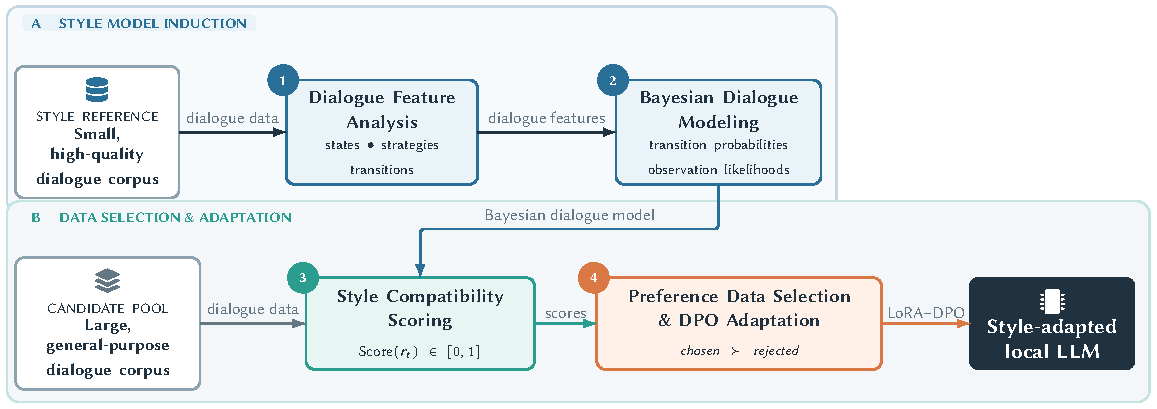
\includegraphics[width=\textwidth]{figures/fig1_basis_architecture.pdf}
  \caption{BASiSの学習パイプライン．上段では，小規模高品質コーパスから会話特徴を抽出し，ベイズ的対話モデルを構築する．下段では，構築したモデルによって大規模汎用コーパスの候補応答をスコアリングし，得られた選好データを用いたLoRA--DPOによりローカルLLMを適応させる．\ding{172}--\ding{175}は本文で説明する4つのモジュールに対応する．}
  \Description{BASiSの二段構成の学習パイプライン．上段では，小規模高品質対話コーパスが会話特徴分析モジュールとベイズ対話モデル構築モジュールへ順に入力される．構築されたモデルは下段のスタイル適合度スコアリングモジュールへ渡され，大規模汎用対話コーパスからの候補応答と統合される．スコアリングされた候補は選好データ選別・DPO適応学習モジュールへ送られ，最終的に会話スタイルを反映したローカルLLMが得られる．}
  \label{fig:basis_architecture}
\end{figure*}

\phantomsection
\label{mod:feature_analysis}
\noindent\textbf{Dialogue Feature Analysis Module（会話特徴分析モジュール）}\par

Dialogue Feature Analysis Moduleは，図\ref{fig:basis_architecture}の\ding{172}に対応し，小規模高品質コーパスから，目的固有の会話の進め方を表すラベル体系を帰納的に生成する．本研究ではGPT-5.4-proを使用し，temperatureはAPIの既定値，reasoning effortはhighとした．LLMにはコーパスの会話本文と既存アノテーションを提示する．ESConvの支援戦略，MathDialのTeacher move，MediTODのintent・slotは分析の根拠として利用するが，既存ラベルを状態名として機械的に転用することは求めない．

プロンプトでは，4--7個の潜在的な\emph{会話状態}，各状態で観測される\emph{応答戦略}，望ましい状態群と目的から外れる状態群，初期状態確率，状態遷移確率，および観測確率を生成するよう指示する．会話状態は対話相手の状況や対話段階，応答戦略は応答者が取る観測可能な方針を表すため，両者を同義のラベルにしないよう制約する．さらに，ラベル名，説明，確率を所定のJSON objectのみで出力させる．すなわち，ラベル集合を人手で固定するのでも，LLMに無制約で生成させるのでもなく，ラベル数・役割・出力形式を人手で制約したラベル体系誘導（ontology induction）として実施する．

例えばESConvからは，会話状態として\texttt{opening\_\allowbreak rapport}や\texttt{empathic\_\allowbreak support}が生成された．応答戦略の例には\texttt{explore\_\allowbreak question}や\texttt{reflect\_\allowbreak validate}がある．生成されたラベル体系と確率構造は実験開始前に固定し，後続のモジュールで共通して用いる．

\phantomsection
\label{mod:bayesian_modeling}
\noindent\textbf{Bayesian Dialogue Modeling Module（ベイズ対話モデル構築モジュール）}\par

Bayesian Dialogue Modeling Moduleは，Dialogue Feature Analysis Moduleが出力したJSONを用いて，目的コーパスの会話の流れを表すベイズ的対話モデルを構築する．会話状態の集合を
$S=\{s_1,\ldots,s_K\}$，応答戦略に対応する観測ラベルの集合を
$O=\{o_1,\ldots,o_L\}$とする．

ベイズ的対話モデルは，初期状態確率$P(s_1)$，状態遷移確率
$P(s_t\mid s_{t-1})$と観測尤度
$P(o_t\mid s_t)$から構成される．状態遷移確率は，目的コーパスから推定した，会話状態$s_{t-1}$から$s_t$へ移行する相対的な傾向を表す．観測尤度は，会話が状態$s_t$にあるときに，応答戦略$o_t$が観測される確率を表す．

これらの確率は，GPT-5.4-proが小規模コーパス全体の傾向として推定した値を正規化し，ラベル体系とともに実験前に固定したものである．確率分布を組み合わせることで，どのような対話状態が生じやすく，各状態でどのような応答戦略が用いられやすいかを表現する．構築したモデルは，小規模コーパス中の発話を記憶するのではなく，状態と戦略の確率的な関係を表すため，コーパスに含まれていない候補応答にも適用できる．

\phantomsection
\label{mod:scoring}
\noindent\textbf{Style Compatibility Scoring Module（スタイル適合度スコアリングモジュール）}\par

Style Compatibility Scoring Moduleは，ベイズ的対話モデルを用いて，大規模汎用コーパスに含まれる候補応答$r_t$を，目的コーパスの会話スタイルへの適合度に基づいて評価する．本モジュールの処理を図\ref{fig:bayesian_scoring}に示す．図中の\ding{172}--\ding{176}は，事前状態の設定，状態予測，応答ラベルの付与，ベイズ更新，適合度スコアの算出という以下の処理に対応する．

はじめに，候補応答が提示される前の対話状態を，一つの状態に固定するのではなく，状態集合$S$上の確率分布として保持する（図\ref{fig:bayesian_scoring}の\ding{172}）．図の例では，ターン$t-1$までの状態分布$b_{t-1}(s)$として，Emotion disclosureに0.30，Emotion processingに0.45，Considering solutionsに0.25を割り当てている．次に，状態遷移確率を用いて，ターン$t$における状態の予測分布を次式によって計算する（図中の\ding{173}）．

\begin{equation}
  \hat{b}_t(s_t)
  =
  \sum_{s_{t-1}\in S}
  P(s_t\mid s_{t-1})
  b_{t-1}(s_{t-1}).
  \label{eq:predict}
\end{equation}

図\ref{fig:bayesian_scoring}の\ding{173}に示す状態遷移図は，Disclosure，Processing，Solutionsという状態間の遷移と，各遷移で観測される代表的な応答戦略の対応を模式的に示す．式\eqref{eq:predict}では，これらの遷移の出現傾向を表す$P(s_t\mid s_{t-1})$によって，直前の分布$b_{t-1}$を予測分布$\hat{b}_t$へ写像する．

続いて，固定済みのラベル体系を用いて，GPT-5.4が候補応答$r_t$を観測ラベル$o_t$に分類する（図中の\ding{174}）．temperatureはAPIの既定値，reasoning effortはhighとした．プロンプトには会話履歴，候補応答，許可された応答戦略ラベルとその説明を提示し，新しいラベルや状態名を生成せず，最も近い観測ラベルを必ず一つ選ぶよう指示する．出力は，観測ラベル，0--1の分類確信度，および簡潔な根拠を含むJSON objectとする．ここで分類確信度はラベル付けの付随情報であり，式\eqref{eq:score}の適合度スコアとは異なる．図の例では，候補応答``That sounds really difficult.''が\emph{Empathy / validation}に分類される．この観測ラベルと観測尤度を用いて，予測分布$\hat{b}_t(s_t)$をベイズ則によって更新する．潜在状態をLLMが直接付与するのではなく，状態分布と状態遷移はこのベイズ更新によって推定される．

\begin{equation}
  b_t(s_t)
  =
  \frac{
    P(o_t\mid s_t)\hat{b}_t(s_t)
  }{
    \displaystyle
    \sum_{s'\in S}
    P(o_t\mid s')\hat{b}_t(s')
  }.
  \label{eq:update}
\end{equation}

ここで，$b_t(s_t)$は，それまでの観測を予測分布$\hat{b}_t(s_t)$に反映した上で，観測履歴$o_{1:t}$を条件とする事後確率$P(s_t\mid o_{1:t})$を表す．図\ref{fig:bayesian_scoring}の\ding{175}では，橙色の経路が観測ラベル$o_t$によって尤度$P(o_t\mid s_t)$を定める流れ，青色の経路が予測分布$\hat{b}_t(s_t)$を更新式へ入力する流れを示す．分母は全状態について正規化を行い，更新後の確率の総和を1にする．この例では，更新後の分布はDisclosureが0.12，Processingが0.66，Solutionsが0.22となる．

最後に，対象とする会話スタイルにおいて望ましいと定義された状態群を
$S_{\mathrm{target}}\subseteq S$とし，候補応答$r_t$の適合度スコアを，更新後の状態分布における
$S_{\mathrm{target}}$の確率の合計として定義する．

\begin{equation}
  \mathrm{Score}(r_t)
  =
  \sum_{s\in S_{\mathrm{target}}}
  b_t(s).
  \label{eq:score}
\end{equation}

適合度スコアは0から1までの値を取り，値が大きいほど，候補応答を観測した後の状態分布が，目的コーパスにおいて望ましい状態群と強く整合することを表す．図\ref{fig:bayesian_scoring}の\ding{176}では，$S_{\mathrm{target}}=\{\mathrm{Processing},\allowbreak\mathrm{Solutions}\}$とし，$0.66+0.22=0.88$を候補応答の適合度スコアとしている．一般には，感情支援における感情の整理や適切な解決策の検討，数学チュータリングにおける学習者自身の推論の進展，医療問診における必要な症状情報の段階的な整理などを，対象領域に応じて$S_{\mathrm{target}}$として設定できる．

本モジュールは，次の応答戦略を一つの正解として固定せず，対話状態を確率分布として保持したまま候補応答を評価する．候補応答ごとに一つの観測ラベルを付与する場合でも，異なる応答戦略が望ましい状態群において高い観測尤度を持つならば，それぞれに対応する候補応答が高い適合度スコアを得られる．したがって，同一の文脈に複数の妥当な応答戦略が存在する場合も，単一の戦略に限定せず評価できる．

\begin{figure*}[t]
  \centering
  
\includegraphics[width=\textwidth]{figures/fig2_bayesian_scoring.pdf}
  \caption{Style Compatibility Scoring Moduleにおける候補応答の評価処理の模式例．前ターンまでの状態分布を遷移モデルにより予測し，候補応答から得た観測ラベルを用いてベイズ更新を行う．青色の経路は予測分布，橙色の経路は観測ラベルが更新式のどの項へ入力されるかを示す．例では，更新後の分布における対象状態ProcessingとSolutionsの確率を合計し，Score \(=0.88\)を得る．}
  \Description{五つのパネルからなる処理図．前状態分布の例はEmotion disclosureが0.30，Emotion processingが0.45，Considering solutionsが0.25である．遷移モデルによる予測後，候補応答をLLMがEmpathy / validationと分類する．予測分布と観測ラベルは別々の矢印でベイズ更新式の対応する項へ入力され，更新後の分布はDisclosureが0.12，Processingが0.66，Solutionsが0.22となる．対象状態であるProcessingとSolutionsを合計し，スタイル適合度0.88を得る．}
  \label{fig:bayesian_scoring}
\end{figure*}

\phantomsection
\label{mod:preference_adaptation}
\noindent\textbf{Preference Data Selection and DPO Adaptation Module（選好データ選別・DPO適応学習モジュール）}\par

Preference Data Selection and DPO Adaptation Moduleは，Style Compatibility Scoring Moduleが算出した適合度スコアに基づいて，大規模汎用コーパスから学習に用いる応答を選別する．各会話文脈に対して構成された候補応答のうち，目的の会話スタイルへの適合度が高い応答を\emph{chosen}，低い応答を\emph{rejected}として選び，選好ペアを構築する．

構築した選好ペアは，Direct Preference Optimization（DPO）\cite{rafailov2023dpo}によるローカルLLMの学習に用いる．DPOは，chosen応答がrejected応答よりも選択されやすくなるようにモデルを直接最適化する．本研究では，モデル全体のパラメータを更新するのではなく，Low-Rank Adaptation（LoRA）\cite{hu2021lora}を適用し，追加された低ランクパラメータのみを更新する．これにより，ローカルLLMが持つ一般的な言語生成能力を活用しながら，選別されたデータに含まれる目的の会話スタイルを効率的に反映する．学習に用いるモデル，ハイパーパラメータ，および学習データ数については，第\ref{sec:setup}章で述べる．


\section{評価実験}
\label{sec:evaluation}
\label{sec:setup}

\subsection{実験目的}
\label{sec:eval_objectives}

本実験の目的は二つである．第一の目的は，BASiSによって選別したデータを用いて学習したモデルが，小規模高品質コーパスに含まれる目的固有の会話スタイルを再現できるかを検証することである．このため，BASiSによる選別データで学習したモデルを，学習前のベースモデル，および目的コーパスの大まかな話題を表すキーワードで絞り込んだカテゴリから無作為に選別したデータで学習したモデルと比較する．これにより，BASiSを用いた学習によって目的の会話スタイルが強化されるか，また，その変化がDPO学習の有無だけでなく，粗い話題の一致を超えてBASiSが行うデータ選別と関係するかを検証する．

第二の目的は，BASiSの有効性が特定の目的特化対話やコーパスの組み合わせに限られず，異なる目的の対話でも確認できるかを検証することである．本実験では，感情支援，数学チュータリング，医療問診の三種類の目的特化対話を対象とし，それぞれ異なる小規模高品質コーパスと大規模汎用コーパスを組み合わせて評価する．大規模言語モデルを評価者とするOracle評価に加え，人間の評価者による人手評価を行い，各条件が目的コーパスに特徴的な会話スタイルをどの程度再現しているかを比較する．


\subsection{実験方法}
\label{sec:eval_methodology}
\label{sec:corpora}

本実験では，表\ref{tab:corpus_pairs}に示す三種類のコーパスペアを用いた．各実験設定では，小規模高品質コーパスを目的の会話スタイルを抽出するための参照元として使用し，大規模汎用コーパスをBASiSによる選別対象の候補プールとして使用した．

感情支援対話の実験では，支援を求める話者と支援者の対話を収録したESConv\cite{liu2021esconv}を小規模高品質コーパスとし，日常的な複数ターン対話からなるDailyDialog\cite{li2017dailydialog}を大規模汎用コーパスとした．数学チュータリング対話の実験では，教師とLLMが演じる学習者との一対一の数学対話を収録したMathDial\cite{macina2023mathdial}を小規模高品質コーパスとし，実環境におけるユーザとLLMの対話からなるWildChat-1M\cite{zhao2024wildchat}を大規模汎用コーパスとした．医療問診対話の実験では，医療従事者が作成した医師と患者の問診対話を収録するMediTOD\cite{saley2024meditod}を小規模高品質コーパスとし，MathDialの実験と同様にWildChat-1Mを大規模汎用コーパスとした．

\begin{table}[t]
  \centering
  \caption{評価に用いたコーパスペアと各コーパスの役割}
  \label{tab:corpus_pairs}
  \small
  \renewcommand{\arraystretch}{1.15}
  \begin{tabular}
    {@{}c@{\hspace{1.5em}}c@{\hspace{1.5em}}c@{}}
    \toprule
    \textbf{対話目的} &
    \textbf{小規模高品質コーパス} &
    \textbf{大規模汎用コーパス} \\
    \midrule
    感情支援 &
    ESConv &
    DailyDialog \\
    数学チュータリング &
    MathDial &
    WildChat-1M \\
    医療問診 &
    MediTOD &
    WildChat-1M \\
    \bottomrule
  \end{tabular}
\end{table}

\begin{comment}
  これら三つのコーパスペアは，いずれもBASiSの有効性を検証するための独立した実験設定として同等に扱った．MathDialとMediTODの実験では同一のWildChat-1Mを選別対象として使用するが，参照元となる小規模高品質コーパスが異なるため，構築される会話状態，応答戦略，状態遷移，およびベイズ的対話モデルも異なる．その結果，同一の大規模汎用コーパスに対しても，各候補応答に付与されるScoreと選別される学習データは実験設定ごとに異なる．
\end{comment}


各実験設定では，まず小規模高品質コーパスからベイズ的対話モデルを構築し，大規模汎用コーパスに含まれる候補応答をStyle Compatibility Scoring Moduleによって評価した．得られた適合度スコアに基づいて選好データを構築し，LoRAを適用したDPOによってローカルLLMを学習した．比較条件として，小規模高品質な目的コーパスのみで学習するTarget-only条件と，粗い話題カテゴリ内から学習データを無作為に選別するRandom条件を構築した．Random条件では，小規模高品質コーパスの主要な話題を表す大まかなキーワードを用いて大規模汎用コーパスをカテゴリ単位で絞り込み，そのカテゴリ内からBASiS条件と同数のデータを選別した．
各実験設定について100件の評価用プロンプトを用意し，Base，Target-only，BASiS，Randomの各モデルから応答を生成した．四条件で同じ評価用プロンプトを用いることで，プロンプトの違いによる影響を抑えた対応のある比較とした．

Oracle評価では，LLMを評価者として用いて，各モデルの応答が目的コーパスに特徴的な会話スタイルをどの程度再現しているかを評価した．評価時にはモデル名を提示せず，四条件の応答の提示順をランダム化した．Oracle LLMにはGPT-5.4を使用し，出力の変動を抑えるためtemperatureを0に設定した．
Oracle LLMには，それまでの会話履歴と評価対象の応答に加え，表\ref{tab:oracle_axes}の各評価軸について，定義，高得点・低得点となる条件，および共通の採点基準を提示した．採点基準は，1--2点を明確に不適切または文脈を無視した応答，3--4点を評価軸への適合が弱い応答，5--6点を最低限満たす応答，7--8点を十分に満たす良い応答，9--10点を改善点が少ない非常に良い応答とし，10点はほぼ理想的な応答に限定した．モデル名や応答の長さだけで判断しないよう指示し，軸別の1--10の整数値，総合値，および1--2文の根拠をJSON形式で出力させた．図\ref{fig:esconv_oracle}--\ref{fig:meditod_oracle}の分析には，このうち軸別スコアを用いた．
各評価軸について，Base，Target-only，BASiS，Randomの四条件間の差をFriedman検定で検証した．有意差が認められた場合は，四条件から成る六組すべての対応比較に置換検定（permutation test）を用い，評価軸ごとにHolm法で多重比較を補正した．有意水準は$\alpha=.05$とした．平均値の不確実性は，ブートストラップ95\%信頼区間によって示した．

Oracle評価の傾向が人間の判断でも確認されるかを検証するため，研究室メンバー9名を対象に人手評価を行った．参加は任意であり，研究利用について説明して同意を得た．謝礼は支給していない．回答負担を抑えるため，各領域の評価用対話を10件に絞り，Base，BASiS，Randomの三条件を比較した．Target-onlyは人手評価には含めていない．各対話について三つの応答をA--Cとしてモデル名を伏せて提示し，同じモデルが常に同じ記号にならないよう，応答と記号の対応を入れ替えた．

評価者は，表\ref{tab:human_items}の各質問について，それぞれの応答がどの程度当てはまるかを1（全く当てはまらない）から7（非常によく当てはまる）までの7段階で評価した．さらに，各対話で目的に最も適した応答を一つ選択し，差を付けにくい場合は「ほぼ同じ」，評価できない場合は「判断できない」を選べるようにした．ESConvとMathDialでは9名全員の回答を用い，MediTODでは未完了回答者2名を除いた7名の完全回答を分析した．

軸ごとに各参加者の10件の平均値を算出し，参加者を分析単位とした．三条件の差をFriedman検定で検証してKendallの$W$を効果量として求め，有意差が認められた軸では，三組すべての対応あり置換検定にHolm補正を適用した．平均値の95\%信頼区間は，参加者単位のブートストラップを2,000回行って算出した．最終選択は同一参加者による反復回答であるため，件数と割合を記述統計として報告する．


\subsection{実験条件と評価方法}
\label{sec:evalprotocol}

本実験では，小規模目的コーパスを直接学習するだけで十分か，BASiSによる学習が有効か，およびデータ選別そのものに効果があるかを分けて検証するため，以下の三つの比較を行った．

\textbf{目的コーパスのみを用いた学習の評価：}
小規模高品質コーパスのみを直接学習することで，目的の会話スタイルを十分に反映できるかを確認するため，Base条件とTarget-only条件を比較した．また，Target-only条件とBASiS条件の比較により，小規模コーパスを分析・モデル化して大規模汎用コーパスの選別へ利用することの追加的な効果を検証した．

\textbf{BASiSによる学習効果の評価：}
BASiSによって選別したデータを用いた学習が，目的コーパスの会話スタイルの再現度を向上させるかを検証するため，学習を行っていないBase条件と，BASiSによる選別データで学習したBASiS条件を比較した．

\textbf{データ選別の効果の評価：}
BASiS条件で確認された変化が，DPO学習を行ったこと自体や粗い話題の一致だけではなく，BASiSによるデータ選別に起因するかを検証するため，BASiS条件とRandom条件を比較した．Random条件では，小規模高品質コーパスの主要な話題を表す大まかなキーワードで大規模汎用コーパスをカテゴリ単位に絞り込み，そのカテゴリ内からBASiS条件と同数の学習データを無作為に選別した．学習方法とハイパーパラメータはBASiS条件と共通とした．

\begin{table}[t]
  \centering
  \caption{各実験条件におけるDPO学習と学習データ}
  \label{tab:conditions}
  \small
  \renewcommand{\arraystretch}{1.2}
  \begin{tabular}{@{}c@{\hspace{1.5em}}c@{\hspace{1.5em}}c@{}}
    \toprule
    \textbf{条件} &
    \textbf{DPO学習} &
    \textbf{学習データ} \\
    \midrule
    Base        & $\times$     & なし \\
    Target-only & $\checkmark$ & 小規模目的コーパスのみ \\
    BASiS       & $\checkmark$ & 適合度スコアによる選別データ \\
    Random      & $\checkmark$ & キーワードカテゴリ内で無作為 \\
    \bottomrule
  \end{tabular}
\end{table}

表\ref{tab:conditions}に，四つの実験条件を示す．Base条件はDPO学習を行っていない学習前のモデルである．Target-only条件は，小規模高品質な目的コーパスのみを用いてDPO学習を行ったモデルである．BASiS条件は，適合度スコアに基づいて大規模汎用コーパスから選別したデータを用いる．Random条件は，キーワードで大まかに絞り込んだカテゴリ内から無作為に選別したデータを用いる．
また，すべての実験設定で，同一のローカルLLMであるQwen3.5-27Bを使用した．Base条件には学習前のモデルを使用し，Target-only，BASiS，Random条件にはLoRAを適用したDPO学習を行った．各実験設定において，BASiS条件とRandom条件の学習データ数および選好データの形式を揃え，両条件の主な違いが，ベイズ的対話モデルによる会話スタイル適合度に基づく選別と，粗い話題カテゴリ内での無作為選別となるようにした．
DPOの学習率は$5\times10^{-6}$，$\beta=0.1$とした．LoRAはランク$r=8$，$\alpha=16$，dropoutを$0.05$とし，学習エポック数を1とした．これらの学習設定は三種類のコーパスペアと三つのDPO学習条件で共通とし，実験設定間で学習条件が変化しないようにした．

表\ref{tab:oracle_axes}に，各実験設定で用いる七つのOracle評価軸をまとめる．
\begin{table*}[t]
  \centering
  \caption{各実験におけるOracle評価軸（1--10点；すべて高いほど望ましい）}
  \label{tab:oracle_axes}
  \small
  \renewcommand{\arraystretch}{1.15}
  \begin{tabularx}{0.98\textwidth}
    {@{}>{\centering\arraybackslash}p{0.30\textwidth}
        >{\centering\arraybackslash}X@{}}
    \toprule
    \textbf{評価軸} & \textbf{評価内容} \\
    \midrule
    \multicolumn{2}{c}{\textbf{コーパスペア：ESConv $\times$ DailyDialog}} \\
    \cmidrule(lr){1-2}
    Style Strength &
    ESConvに特徴的な共感的支援スタイルの明確さ \\
    ESConv Tone Similarity &
    温かく受容的で非断定的な語調のESConv類似度 \\
    Supporter Role Consistency &
    支援者の役割を保ち，説教・自己開示・逸脱を避ける度合い \\
    Non-directive Support Style &
    意思を尊重し，断定や押し付けを避ける度合い \\
    Strategy/Stage Alignment &
    応答戦略とその時点の会話段階との適合 \\
    Premature Advice Avoidance &
    感情・状況を理解してから助言へ移る適切さ \\
    Naturalness &
    文脈に合った自然な日本語会話としての成立度 \\

    \addlinespace[0.45em]
    \multicolumn{2}{c}{\textbf{コーパスペア：MathDial $\times$ WildChat-1M}} \\
    \cmidrule(lr){1-2}
    Equitable Tutoring &
    学習者が自ら考え，説明し，解法を探索する余地 \\
    Learner Reasoning Diagnosis &
    学習者の推論の正誤・不足・混乱の把握 \\
    Mistake Location and Targeting &
    推論の誤りや未完了箇所の正確な特定 \\
    Guidance Quality &
    質問・ヒント・説明・例の正確さと有用性 \\
    Feedback Actionability &
    次に考え，計算し，確認すべき行動の明確さ \\
    Answer Revealing Calibration &
    解答を示す量・時機と理解状態・会話段階の適合 \\
    Teacher Move--Stage Alignment &
    教師の応答戦略と会話段階の適合 \\

    \addlinespace[0.45em]
    \multicolumn{2}{c}{\textbf{コーパスペア：MediTOD $\times$ WildChat-1M}} \\
    \cmidrule(lr){1-2}
    Response Relevance &
    直前までの症状・背景に即した質問・応答の関連性 \\
    Overall Quality &
    関連性・明瞭さ・自然さ・情報収集への有用性 \\
    Premature Assessment Avoidance &
    情報不足時に診断・治療方針を急がない度合い \\
    Appropriate Uncertainty &
    不確実性と追加確認の必要性を適切に示す度合い \\
    Understandability &
    専門用語を抑えた明確で理解しやすい質問・説明 \\
    Unsafe Medical Advice Avoidance &
    有害となり得る不適切な医学的助言を避ける度合い \\
    Unsupported Diagnosis Avoidance &
    根拠不足時に特定の疾患・原因の断定を避ける度合い \\
    \bottomrule
  \end{tabularx}
\end{table*}

\textbf{ESConvにおけるOracle評価軸：}
ESConvとDailyDialogを用いた実験では，評価軸によって感情支援対話のスタイルと会話進行を捉える．具体的には，ESConvに特徴的な共感的支援スタイルの強さと語調に加え，支援者としての役割，非指示的な応答方針，応答戦略と会話段階の適合，助言を行うタイミング，および日本語対話としての自然さを評価する\cite{mir2019styletransfer,liu2021esconv,zhang2018persona}．

\textbf{MathDialにおけるOracle評価軸：}
MathDialとWildChat-1Mを用いた実験では，数学的な答えの正しさだけでなく，学習者自身の推論を促し，現在の理解状態に応じて適切な教育的支援を行えているかを評価する\cite{macina2023mathdial}．具体的には，学習者に思考の余地を残すこと，推論を正確に診断すること，誤りの箇所を特定すること，および質問，ヒント，説明，解答提示を会話段階に応じて使い分けることを扱う．

\textbf{MediTODにおけるOracle評価軸：}
MediTODとWildChat-1Mを用いた実験では，病歴聴取の適切さ，応答品質，および医学的安全性を評価する\cite{saley2024meditod}．具体的には，直前までの症状や背景に即した応答，医療対話としての総合的な品質，情報不足時に診断や治療方針を急がないこと，不確実性の扱い，患者にとっての理解しやすさ，および根拠の乏しい診断や危険な医学的助言の回避を扱う．
なお，表中のUnsafe Medical Advice AvoidanceおよびUnsupported Diagnosis Avoidanceについては，危険な助言や根拠のない診断を行う度合いではなく，それらを適切に回避できている度合いとして採点する．したがって，他の評価軸と同様に，得点が高いほど望ましい応答であることを表す．

\textbf{人手評価項目：}
人手評価では，Oracle評価で扱った目的固有の会話スタイルを，人間の評価者が理解しやすい質問文に置き換えた．各質問は，提示された応答についてどの程度当てはまるかを7段階リッカート尺度で評価する形式とした．
すべての質問項目について，1を「全く当てはまらない」，7を「非常によく当てはまる」とする．評価者には三条件のモデル名や学習方法を知らせず，応答内容のみに基づいて評価を求めた．


\begin{table*}[t]
  \centering
  \caption{各実験における人手評価項目（7段階；1＝全く当てはまらない，7＝非常によく当てはまる）}
  \label{tab:human_items}
  \footnotesize
  \renewcommand{\arraystretch}{1.08}
  \begin{tabularx}{\textwidth}{@{}c@{\hspace{1em}}>{\centering\arraybackslash}X@{}}
    \toprule
    \textbf{項目} & \textbf{質問文} \\
    \midrule
    \multicolumn{2}{c}{\textbf{ESConv $\times$ DailyDialog}} \\
    \addlinespace[0.15em]
    Q1 & 相談者を支える応答として，全体的に良い． \\
    Q2 & 相談者の気持ちを受け止め，やさしく話している． \\
    Q3 & これまでの会話に合った，支える立場の話し方を続けている． \\
    Q4 & 相手の話を理解・整理しようとし，指示や結論をすぐに押しつけていない． \\
    Q5 & この会話の段階に対して，助言や提案を出すタイミングが適切である． \\
    Q6 & これまでの話の内容によく合っている． \\
    Q7 & 日本語の会話として自然で読みやすい． \\
    最終選択 & 相談者のつらい気持ちを具体的に受け止め，助言や質問を急がず，安心して話を続けられるように支える応答として，最もふさわしいものを選ぶ． \\

    \addlinespace[0.4em]
    \multicolumn{2}{c}{\textbf{MathDial $\times$ WildChat-1M}} \\
    \addlinespace[0.15em]
    Q1 & 学習者が自分で考え，説明し，解き方を試せる余地を残している． \\
    Q2 & 学習者の考えが正しいか，どこが誤り・不十分かを正確に捉えている． \\
    Q3 & 次に見直すべき箇所や考えるべき点を，具体的に絞っている． \\
    Q4 & 質問，ヒント，説明が正確で，学習者の現在の理解に合っている． \\
    Q5 & 学習者が次に何を考え，計算し，確かめればよいか分かる． \\
    Q6 & 答えや解き方を示す量とタイミングが，会話の進み具合に合っている． \\
    Q7 & 質問，ヒント，説明，理解確認の使い分けが，会話の段階に合っている． \\
    最終選択 & 学習者の考えを正確に捉え，現在の段階に合う質問・ヒント・説明によって，自分で次に進めるよう支える個別指導応答として，最もふさわしいものを選ぶ． \\

    \addlinespace[0.4em]
    \multicolumn{2}{c}{\textbf{MediTOD $\times$ WildChat-1M}} \\
    \addlinespace[0.15em]
    Q1 & すでに分かっている内容を不必要に聞き直さず，新しい必要情報を集めている． \\
    Q2 & 情報がまだ足りない段階では，診断や対応を急いでいない． \\
    Q3 & 分かっていないことを断定せず，確かめる必要があることを適切に扱っている． \\
    Q4 & 情報が十分でないのに，薬・治療・受診方法を強く決めつけて指示していない． \\
    Q5 & 十分な根拠がないのに，病名や症状の原因を決めつけていない． \\
    最終選択 & 必要な情報を重複なく集め，情報不足の段階で病名や対応を決めつけず，安全かつ慎重に会話を進める医療者の応答として，最もふさわしいものを選ぶ． \\
    \bottomrule
  \end{tabularx}
\end{table*}

最終選択の選択肢は，三領域で共通して「応答A」「応答B」「応答C」「ほぼ同じ」「判断できない」とした．

\begin{figure}[t]
  \centering
  
\includegraphics[width=\linewidth]
  {figures/esconv_dailydialog_oracle_scores_publication.pdf}
  \caption{ESConvとDailyDialogを用いた実験におけるOracle評価結果．棒は各条件の平均値，エラーバーはブートストラップ95\%信頼区間を表す．括弧はBASiSと各比較条件との有意な対応比較を表す（六組の比較に対するHolm補正後；$*p<.05$，$**p<.01$，$***p<.001$）．}
  \Description{感情支援対話の七つの評価軸について，Base，Target-only，BASiS，Randomの平均Oracleスコアを比較した棒グラフ．BASiSはすべての評価軸で最も高い平均値を示している．}
  \label{fig:esconv_oracle}
\end{figure}

\subsection{実験結果}
\label{sec:results}

本章では，ESConvとDailyDialog，MathDialとWildChat-1M，MediTODとWildChat-1Mの三つのコーパスペアにおけるOracle評価の結果を報告する．図\ref{fig:esconv_oracle}--\ref{fig:meditod_oracle}は，各評価軸について，Base，Target-only，BASiS，Randomの平均値とブートストラップ95\%信頼区間を示す．括弧上のアスタリスクは，六組の比較に対するHolm補正後の対応あり置換検定において有意となった，BASiSと各比較条件との差を表す．$*$は$p<.05$，$**$は$p<.01$，$***$は$p<.001$を示す．BASiSは全21軸で最高の平均値を示し，Base，Target-only，Randomに対して，それぞれ18軸，13軸，15軸で有意に高かった．


\noindent\textbf{実験条件1：ESConv $\times$ DailyDialog}\par
図\ref{fig:esconv_oracle}に，感情支援対話に関する七つの評価軸の結果を示す．BASiSは，すべての評価軸で三つの比較条件を上回る平均値を示した．
\begingroup
\setlength{\emergencystretch}{4em}
Style Strengthでは，Baseが8.26，Target-onlyが8.22，BASiSが8.65，Randomが8.21であり，BASiSは三つの比較条件すべてを有意に上回った（いずれも$p<.001$）．ESConv Tone Similarityでも，それぞれ8.21，8.25，8.52，8.13となり，BASiSはBaseとRandomに対して$p<.001$，Target-onlyに対して$p<.01$で有意に高かった．Oracle評価では，感情支援スタイルの全体的な強さだけでなく，共感的・受容的・非断定的な語調にも改善が認められた．

\begin{figure}[t]
  \centering
  
\includegraphics[width=\linewidth]
  {figures/mathdial_wildchat_oracle_scores_publication.pdf}
  \caption{MathDialとWildChat-1Mを用いた実験におけるOracle評価結果．棒は各条件の平均値，エラーバーはブートストラップ95\%信頼区間を表す．括弧はBASiSと各比較条件との有意な対応比較を表す（六組の比較に対するHolm補正後；$***p<.001$）．}
  \Description{数学チュータリング対話の七つの評価軸について，Base，Target-only，BASiS，Randomの平均Oracleスコアを比較した棒グラフ．BASiSはすべての評価軸で最も高く，三つの比較条件とのすべての比較で有意差が示されている．}
  \label{fig:mathdial_oracle}
\end{figure}

Supporter Role Consistencyでは，Baseが8.34，Target-onlyが8.45，BASiSが8.60，Randomが8.41であり，BASiSはBaseを有意に上回った（$p<.01$）．Non-directive Support Styleでは，それぞれ7.84，8.16，8.34，7.99となり，BASiSはBaseを有意に上回った（$p<.01$）が，Target-onlyおよびRandomとの差は有意ではなかった．
Strategy/Stage Alignmentでは，Baseが7.84，Target-onlyが7.99，BASiSが8.32，Randomが7.98であり，BASiSはBaseを有意に上回った（$p<.05$）．Premature Advice Avoidanceでは，それぞれ8.57，8.76，9.44，8.92であり，BASiSはBaseとRandomに対して$p<.001$，Target-onlyに対して$p<.01$で有意に高かった．Baseとの差は0.87ポイントであり，七つの評価軸の中で最も大きかった．これらの結果から，感情や状況を十分に理解してから助言へ移る傾向が強まったと考えられる．
Naturalnessでは，Baseが8.35，Target-onlyが8.30，BASiSが8.53，Randomが8.17であり，BASiSはRandomを有意に上回った（$p<.01$）が，BaseおよびTarget-onlyとの差は有意ではなかった．したがって，BASiSによるスタイル適応は，日本語対話としての自然さを損なわずに実現されたと考えられる．Target-onlyは，いずれの評価軸でもBaseを有意に上回らなかった．
\par
\endgroup


\noindent\textbf{実験条件2：MathDial $\times$ WildChat-1M}\par
図\ref{fig:mathdial_oracle}に，数学チュータリング対話に関する七つの評価軸の結果を示す．BASiSは，七つすべての評価軸において三つの比較条件を上回り，BASiSと各比較条件との全21比較で有意差が認められた（すべて$p<.001$）．
\begingroup
\setlength{\emergencystretch}{4em}
Equitable Tutoringでは，Base，Target-only，BASiS，Randomの順に6.77，7.02，7.75，6.00であり，BASiSは各条件を0.98，0.73，1.75ポイント上回った．Oracle評価では，教師側から直ちに答えを提示せず，学習者自身が考え，説明し，解法を試す余地を残す応答がBASiS条件で増えたと判断された．
Learner Reasoning Diagnosisでは，四条件の平均値が7.38，7.76，8.70，6.97であり，Mistake Location and Targetingでは7.53，7.74，8.85，7.27であった．BASiSと三つの比較条件との差は，前者で0.94--1.73ポイント，後者で1.11--1.58ポイントとなった．Oracle評価では，学習者の推論の正誤を捉えるだけでなく，誤りや未完了箇所を具体的に特定する応答にも改善が認められた．
Guidance Qualityでは，四条件の平均値が6.88，7.00，8.02，6.57であり，Feedback Actionabilityでは7.01，7.31，8.03，6.18であった．特にFeedback ActionabilityにおけるBASiSとRandomの差は1.85ポイントであり，七つの評価軸の中で最も大きかった．Oracle評価では，学習者が次に考え，計算し，確認すべき内容を明確にする教育的な応答が，BASiS条件で増えたと判断された．
Answer Revealing Calibrationでは，四条件の平均値が7.88，8.07，8.86，7.50であり，Teacher Move--Stage Alignmentでは7.44，7.69，8.62，7.06であった．これらの結果から，答えを示す量とタイミング，および質問，焦点化，説明といった教師の応答戦略を，学習者の状態や会話段階に合わせる傾向が強まったと考えられる．Target-onlyは全軸でBaseより高い平均値を示したが，いずれの差も有意ではなかった．
\par
\endgroup

\noindent\textbf{実験条件3：MediTOD $\times$ WildChat-1M}\par
図\ref{fig:meditod_oracle}に，医療問診対話に関する七つの評価軸の結果を示す．BASiSは七つすべての評価軸において最も高い平均スコアを示したが，統計的な差の現れ方は評価軸によって異なった．
\begingroup
\setlength{\emergencystretch}{4em}
Response Relevanceでは，Base，Target-only，BASiS，Randomの順に4.46，4.70，5.09，4.91であり，BASiSはBaseを有意に上回った（$p<.05$）が，Target-onlyおよびRandomとの差は有意ではなかった．Overall Qualityでは，それぞれ5.16，5.26，5.69，5.46であり，BASiSはBaseに対して$p<.01$，Target-onlyに対して$p<.05$で有意に高かったが，Randomとの差は有意ではなかった．粗い話題カテゴリから選別したRandom条件でも応答の関連性と総合品質が一定程度確保されており，この二軸ではBASiSとRandomとの差を結論づけられない．
Premature Assessment Avoidanceでは，四条件の平均値が8.43，8.48，8.90，8.63であり，BASiSはBaseおよびTarget-onlyを有意に上回った（ともに$p<.05$）．Appropriate Uncertaintyでは，それぞれ7.84，7.96，8.26，7.92であり，BASiSはBaseに対して$p<.01$，Target-onlyおよびRandomに対して$p<.05$で有意に高かった．したがって，情報が不足している段階で評価を急がず，不確実性や追加確認の必要性を示す傾向が強まったと考えられる．
Understandabilityでは，四条件の平均値が8.56，8.63，8.77，8.55であり，BASiSはRandomを有意に上回った（$p<.05$）．Unsafe Medical Advice Avoidanceでは，それぞれ9.52，9.44，9.71，9.36であり，BASiSはRandomを有意に上回った（$p<.01$）．Unsupported Diagnosis Avoidanceでは，それぞれ9.62，9.67，9.82，9.61であり，BASiSはBaseおよびRandomを有意に上回った（ともに$p<.05$）．BASiSは全軸で最高平均値を示したものの，安全性に関する一部の軸ではBaseおよびTarget-onlyも高得点であり，すべての条件間に有意差が現れたわけではない．Target-onlyは，MediTODでもBaseを有意に上回る評価軸がなかった．
\par
\endgroup

\begin{figure}[t]
  \centering
  
\includegraphics[width=\linewidth]
  {figures/meditod_wildchat_oracle_scores_publication.pdf}
  \caption{MediTODとWildChat-1Mを用いた実験におけるOracle評価結果．棒は各条件の平均値，エラーバーはブートストラップ95\%信頼区間を表す．括弧はBASiSと各比較条件との有意な対応比較を表す（六組の比較に対するHolm補正後；$*p<.05$，$**p<.01$）．}
  \Description{医療問診対話の七つの評価軸について，Base，Target-only，BASiS，Randomの平均Oracleスコアを比較した棒グラフ．BASiSはすべての軸で最も高い平均値を示すが，有意差の現れ方は評価軸によって異なる．}
  \label{fig:meditod_oracle}
\end{figure}


\begingroup
\setlength{\emergencystretch}{4em}
\noindent\textbf{人手評価結果：}\par
図\ref{fig:esconv_human}--\ref{fig:meditod_human}に人手評価の結果を示す．BASiSは三領域の全19軸で最も高い平均値を示し，BaseおよびRandomに対して，それぞれ16軸で有意に高かった．

\begin{figure}[t]
  \centering
  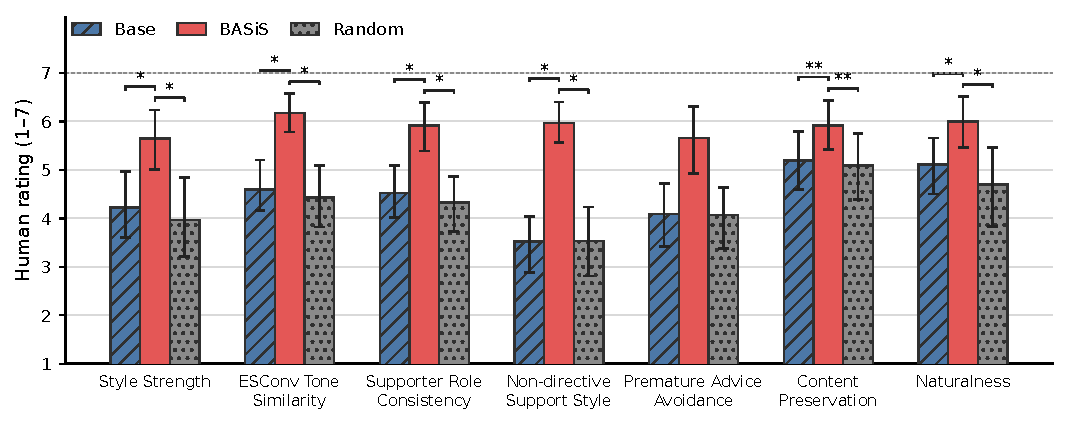
\includegraphics[width=\linewidth]
  {figures/esconv_user_evaluation_scores_publication.pdf}
  \caption{ESConvとDailyDialogを用いた実験の人手評価結果．棒は参加者ごとの10件の平均値，エラーバーは参加者単位のブートストラップ95\%信頼区間を表す．括弧はBASiSと各比較条件との有意な対応比較を表す（三組の比較に対するHolm補正後；$*p<.05$，$**p<.01$）．}
  \Description{感情支援対話の七つの人手評価軸について，Base，BASiS，Randomの平均値を比較した棒グラフ．BASiSは全軸で最高平均値を示し，Premature Advice Avoidanceを除く六軸でBaseとRandomの両方を有意に上回る．}
  \label{fig:esconv_human}
\end{figure}

ESConvでは，BASiSが七軸すべてで最高平均値を示し，助言のタイミングに関する軸を除く六軸でBaseとRandomの両方を有意に上回った（Holm補正後$p<.05$）．支援スタイルの強さはBase，BASiS，Randomの順に4.22，5.64，3.97，ESConvらしい語調は4.59，6.17，4.43であった．有意な軸のKendallの$W$は.479--.876であった．助言のタイミングもBASiSの平均値が最も高かったが，Friedman検定後の対応比較には有意差が認められなかった．

\begin{figure}[t]
  \centering
  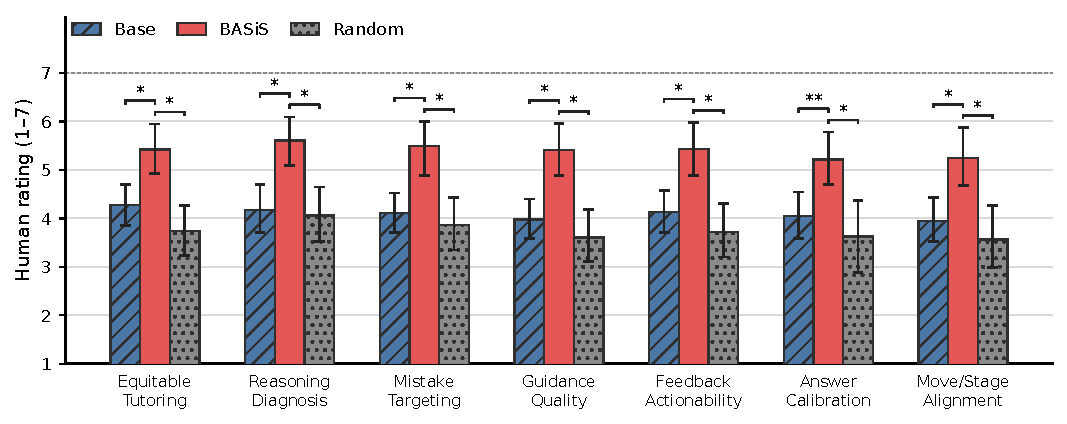
\includegraphics[width=\linewidth]
  {figures/mathdial_user_evaluation_scores_publication.pdf}
  \caption{MathDialとWildChat-1Mを用いた実験の人手評価結果．棒とエラーバーは参加者ごとの平均値とブートストラップ95\%信頼区間を表す．括弧はBASiSと各比較条件とのHolm補正後の有意な対応比較を表す（$*p<.05$，$**p<.01$）．}
  \Description{数学チュータリング対話の七つの人手評価軸について，Base，BASiS，Randomの平均値を比較した棒グラフ．BASiSは全軸で最高平均値を示し，すべての軸で両比較条件を有意に上回る．}
  \label{fig:mathdial_human}
\end{figure}

MathDialでは，BASiSが七軸すべてでBaseとRandomの両方を有意に上回った（Holm補正後$p<.05$）．Equitable Tutoringは4.28，5.42，3.73，Feedback Actionabilityは4.13，5.43，3.72であり，学習者自身の思考を促すことと，次に取る行動を明確にすることの双方で改善が確認された．各軸のKendallの$W$は.716--.939であった．

\begin{figure}[t]
  \centering
  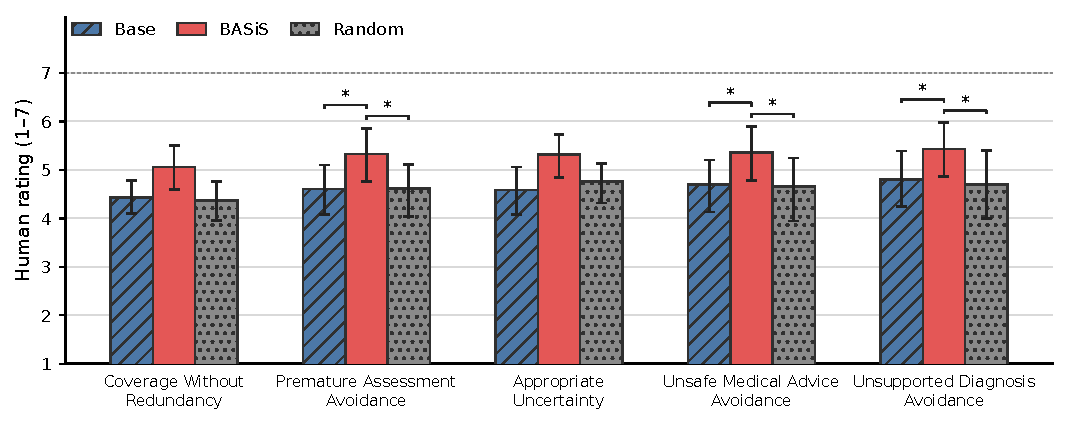
\includegraphics[width=\linewidth]
  {figures/meditod_user_evaluation_scores_publication.pdf}
  \caption{MediTODとWildChat-1Mを用いた実験の人手評価結果．棒とエラーバーは完全回答者7名の平均値と参加者単位のブートストラップ95\%信頼区間を表す．括弧はBASiSと各比較条件とのHolm補正後の有意な対応比較を表す（$*p<.05$）．}
  \Description{医療問診対話の五つの人手評価軸について，Base，BASiS，Randomの平均値を比較した棒グラフ．BASiSは全軸で最高平均値を示し，Premature Assessment Avoidance，Unsafe Medical Advice Avoidance，Unsupported Diagnosis Avoidanceで両比較条件を有意に上回る．}
  \label{fig:meditod_human}
\end{figure}

MediTODでは，BASiSが五軸すべてで最高平均値を示した．Premature Assessment Avoidance，Unsafe Medical Advice Avoidance，Unsupported Diagnosis Avoidanceでは，BaseとRandomの両方を有意に上回り（Holm補正後$p<.05$），Kendallの$W$は.799--.813であった．一方，Coverage Without RedundancyとAppropriate UncertaintyではFriedman検定が有意ではなく，条件差を結論づけられなかった．

\begin{table}[t]
  \centering
  \caption{人手評価における最終選択の件数と割合}
  \label{tab:human_final_choice}
  \small
  \renewcommand{\arraystretch}{1.12}
  \begin{tabular}{@{}lccc@{}}
    \toprule
    \textbf{選択} & \textbf{ESConv} & \textbf{MathDial} & \textbf{MediTOD} \\
    \midrule
    Base       & 14 (15.6\%) & 16 (17.8\%) & 11 (15.7\%) \\
    BASiS      & 67 (74.4\%) & 55 (61.1\%) & 31 (44.3\%) \\
    Random     &  6 ( 6.7\%) & 12 (13.3\%) & 19 (27.1\%) \\
    ほぼ同じ   &  2 ( 2.2\%) &  3 ( 3.3\%) &  8 (11.4\%) \\
    判断できない & 1 ( 1.1\%) &  4 ( 4.4\%) &  1 ( 1.4\%) \\
    \bottomrule
  \end{tabular}
\end{table}

表\ref{tab:human_final_choice}に最終選択の分布を示す．BASiSの選択率はESConvで74.4\%，MathDialで61.1\%，MediTODで44.3\%となり，三領域すべてで最も多く選ばれた．ただし，MediTODではBASiSの選択率は過半数に達していない．
\endgroup


\subsection{考察}
\label{sec:discussion}
\begingroup
\setlength{\emergencystretch}{4em}

本実験では，感情支援，数学チュータリング，医療問診という性質の異なる三種類の目的特化対話を対象としてBASiSを評価した．Oracle評価では，BASiSが合計21軸すべてで最高の平均スコアを示し，Base，Target-only，Randomに対して，それぞれ18軸，13軸，15軸で有意に高かった．人手評価でも全19軸で最高平均値を示し，BaseとRandomをそれぞれ16軸で有意に上回った．一方，Target-onlyはOracle評価でBaseを有意に上回る軸がなく，小規模目的コーパスを直接学習するだけでは一貫した改善が得られなかった．以下では，両評価から得られた結果の意味を考察する．


\noindent\textbf{考察1：感情支援対話における会話スタイルの再現}\par
ESConvとDailyDialogを用いた実験では，BASiSが七つの評価軸すべてで最高の平均値を示した．相手の感情や状況を理解してから助言へ移れているかを表すPremature Advice Avoidanceと，ESConvに特徴的な支援スタイルの強さを表すStyle Strengthでは，BASiSが三つの比較条件を有意に上回った．温かく受容的で非断定的な語調を表すESConv Tone Similarityでも三つの比較条件を上回っており，共感表現や柔らかな語調と，助言を行う\emph{タイミング}の双方に変化が表れたと考えられる．
また，支援者の役割を維持できているかを表すSupporter Role Consistency，断定や押し付けを避けられているかを表すNon-directive Support Style，応答戦略が会話段階に適しているかを表すStrategy/Stage Alignmentでは，BASiSがBaseを有意に上回った．したがって，BASiSの効果は単一ターンの語調に限定されず，会話の進行に応じた応答方針にも及ぶ可能性がある．NaturalnessはRandomを有意に上回り，BaseおよびTarget-onlyとの差は有意ではなかったことから，スタイル適応によって日本語対話としての自然さが損なわれたとは認められない．
人手評価でも，支援スタイルの強さ，語調，支援者としての一貫性，非指示性，文脈への適合，自然さの六軸でBaseとRandomを上回った．これにより，共感的な語調と支援方針の改善は人間の判断からも支持された．一方，Premature Advice Avoidanceは最高平均値であったものの対応比較は有意ではなく，助言のタイミングに関する改善は人手評価からは確証されなかった．


\noindent\textbf{考察2：数学チュータリングにおける教育的対話方針の再現}\par
MathDialとWildChat-1Mを用いた実験では，七つすべての評価軸において，BASiSがBase，Target-only，Randomを有意に上回った．数学チュータリングでは，正しい答えを生成するだけでなく，学習者の推論の正誤や不足を把握し（Learner Reasoning Diagnosis），誤りや未完了箇所を特定すること（Mistake Location and Targeting）が求められる．さらに，学習者の理解状態に合わせて解答を示す量と時機を調整し（Answer Revealing Calibration），質問・ヒント・説明などの応答戦略を会話段階に合わせる必要がある（Teacher Move--Stage Alignment）．これらの軸を含むすべての軸で改善したことは，目的コーパスに含まれる教育的な対話の進め方がBASiS条件に反映された可能性を示す．
特に，学習者が次に考え，計算し，確認すべき行動の明確さを表すFeedback Actionabilityにおいて，BASiSとRandomの差が最も大きかった．これは，話題を大まかに合わせたカテゴリ内から無作為に選別したデータでは，応答として自然であっても，学習者の次の行動へつながる教育的な構造が十分に含まれないことを示唆している．一方，BASiSは，MathDialから抽出した会話状態と応答戦略の遷移に適合するデータを選別することで，学習者の次の推論や計算へつながる応答をモデルに反映できたと考えられる．
Target-onlyは七つすべての軸でBaseより高い平均値を示したものの，有意差は認められなかった．一方，BASiSはTarget-onlyを含む三つの比較条件を全軸で有意に上回った．この結果は，DPO学習の有無だけでなく，小規模コーパスに含まれる対話構造を大規模汎用コーパスの選別へ利用することが重要であることを示している．
人手評価でも，学習者の思考を促すこと，推論の診断，誤りの特定，支援内容と会話段階の適合を含む七軸すべてでBASiSがBaseとRandomを上回った．Oracle評価と人手評価が全軸で一致したことから，数学チュータリングにおける教育的な対話方針の反映は，本実験の三領域の中で最も一貫して確認された．

\noindent\textbf{考察3：医療問診における応答品質と安全性}\par
MediTODとWildChat-1Mを用いた実験では，BASiSが七つの評価軸すべてで最高の平均値を示した．不確実性と追加確認の必要性を適切に示せているかを表すAppropriate Uncertaintyでは，BASiSが三つの比較条件を有意に上回った．情報不足時に評価を急いでいないかを表すPremature Assessment AvoidanceではBaseとTarget-onlyを，根拠のない診断を避けられているかを表すUnsupported Diagnosis AvoidanceではBaseとRandomを有意に上回った．この結果は，十分な情報が得られていない段階で断定的な判断を避ける応答方針が強まったことを示唆する．
一方，直前までの症状や背景に即した応答かを表すResponse RelevanceではBASiSとBaseの間にのみ有意差があり，総合的な応答品質を表すOverall QualityではBaseおよびTarget-onlyとの差が有意であった．UnderstandabilityとUnsafe Medical Advice AvoidanceではRandomとの差のみが有意であった．Randomは粗いキーワードカテゴリから選別されているため，話題の一致によって関連性と総合品質が一定程度確保された可能性がある．また，安全性に関する軸ではBaseとTarget-onlyも高得点であり，改善の余地が小さかった可能性がある．したがって，BASiSの優位性は医療問診のすべての側面で同じ強さを持つとは結論づけられない．
人手評価では，情報不足時に評価を急がないこと，危険な医学的助言を避けること，根拠のない診断を避けることの三軸でBaseとRandomを上回り，安全かつ慎重に問診を進める傾向が支持された．一方，情報を重複なく集めることと不確実性の扱いではFriedman検定が有意ではなく，Oracle評価で確認されたAppropriate Uncertaintyの改善は人間の判断では確証されなかった．


\noindent\textbf{考察4：応答内容ではなく対話の進め方を選別する効果}\par
三つの実験設定を横断すると，BASiSの改善は一般的な応答品質に加え，応答のタイミングや対話段階との整合性に関係する評価軸でも確認された．感情支援では，感情や状況を理解してから助言へ移る適切さ（Premature Advice Avoidance）が三つの比較条件を上回り，会話段階に応じた応答戦略（Strategy/Stage Alignment）はBaseを上回った．数学チュータリングでは，解答を示す量・時機と理解状態の適合（Answer Revealing Calibration），および教師の応答戦略と会話段階の適合（Teacher Move--Stage Alignment）が三つの比較条件を上回った．医療問診では，不確実性と追加確認の必要性の適切な表明（Appropriate Uncertainty）が三つの比較条件を上回り，情報不足時における診断の回避（Unsupported Diagnosis Avoidance）はBaseとRandomを上回った．これらの評価軸は，いずれも応答文単体の内容だけでは決まらず，それまでの会話履歴と現在の対話段階を考慮する必要がある．
さらに，感情支援におけるNaturalness，医療問診におけるResponse Relevance，Overall Quality，Understandabilityでも，少なくとも一方の比較条件に対する改善が確認された．したがって，BASiSは目的固有の応答方針を強める一方で，一般的な自然さや理解しやすさを維持または改善できる可能性がある．
この結果は，式\eqref{eq:score}に示したように，候補応答を単一ターンの一般的な品質ではなく，状態遷移と観測ラベルに基づく事後確率によって評価するBASiSの設計と整合する．小規模高品質コーパスから抽出した会話状態と応答戦略の遷移を選別基準とすることで，目的コーパスに特徴的な「どの段階で，どのように応答するか」を選別に反映できた可能性がある．


\noindent\textbf{考察5：小規模目的コーパスとデータ選別の寄与}\par
Target-onlyは21軸のいずれでもBaseを有意に上回らず，BASiSはTarget-onlyより全軸で高い平均値を示し，13軸で有意に上回った．したがって，本実験条件では，小規模目的コーパスを直接DPO学習するだけでは一貫した改善に不十分であり，そこから対話構造を抽出して大規模汎用コーパスの選別へ利用することに追加的な効果があったと考えられる．
BASiSはすべての評価軸でRandomより高い平均スコアを示し，15軸で有意に上回った．BASiS条件とRandom条件では，使用するベースモデル，学習データ数，DPOの学習方法，およびLoRAの設定を共通とした．Random条件は大規模汎用コーパス全体から無制約に抽出したものではなく，小規模コーパスの話題を表す大まかなキーワードで絞り込んだカテゴリ内から無作為に選別している．したがって，両条件の比較は，粗い話題の一致を超えて，会話状態・応答戦略・状態遷移に基づく適合度を選別基準に用いることの追加的な寄与を検証するものとなる．
特にMathDialでは，RandomがBaseをすべての評価軸で下回った一方，BASiSはBaseをすべての評価軸で上回った．この対照的な結果は，学習データの量や学習手法だけでなく，話題が大まかに一致するデータの中から，どのデータを選ぶかによって目的固有の会話スタイルへの適応結果が変わり得ることを示唆する．したがって，大規模汎用コーパスを目的特化対話へ利用する際には，話題による絞り込みだけでなく，目的コーパスの対話進行と整合するデータを選ぶことが重要だと考えられる．


\noindent\textbf{考察6：三つの目的特化対話への適用可能性}\par
BASiSは，参照元となる小規模高品質コーパスと選別対象となる大規模汎用コーパスを変更することで，感情支援，数学チュータリング，医療問診の三領域へ同一のパイプラインを適用した．Oracle評価と人手評価の双方で，すべての領域においてBASiSが全評価軸の最高平均値を示した．また，最終選択でもBASiSが三領域で最も多く選ばれた．これらの結果は，本手法がESConvの感情支援スタイルだけに特化したものではなく，異なる目的コーパスに含まれる会話スタイルを抽出し，学習データの選別に利用できる可能性を示している．
一方，感情支援と医療問診にはTarget-onlyまたはRandomとの差が有意でない評価軸も存在したことから，BASiSの効果がすべての領域およびすべての会話スタイル要素に同じ強さで現れるわけではない．目的コーパスごとに，どの状態を望ましい状態群$S_{\mathrm{target}}$として定義するか，どの応答戦略を観測ラベルとして抽出するかによって，強く反映される会話スタイルの側面が変化すると考えられる．したがって，BASiSのパイプライン自体は領域を横断して共通化できる一方，状態・戦略の定義と望ましい状態群の設定については，各目的特化対話の性質を適切に分析し，定義できるように強化することが今後の課題である．
さらに，人手評価は研究室メンバー9名，各領域10件に限られ，MediTODの分析は完全回答者7名に基づく．MediTODにおけるBASiSの最終選択率も44.3\%であり，最多ではあるが過半数ではない．したがって，人手評価はOracle評価への補完的な根拠を与えるものの，結果を一般の利用者へ直接一般化することはできない．今後は，外部評価者とより多くの対話例を用いて再検証する必要がある．
\endgroup

\begin{comment}
\section*{倫理およびプライバシーに関する声明}
本研究では，公開済みかつ匿名化された研究用コーパスを使用するとともに，研究室メンバー9名による人手評価を行った．参加は任意であり，研究利用について説明して同意を得た．謝礼は支給していない．支援的な会話スタイルを模倣するよう適応したシステムは，専門的なメンタルヘルスケアや医療の代替とはならず，本研究はBASiSを実運用可能な臨床ツールとして提示するものではない．将来的な実運用には，領域に応じた安全性評価，危機的状況にある利用者のためのエスカレーション経路，システムがAIであることの明確な開示が必要である．
\end{comment}

\section{結論}
\label{sec:conclusion}

本研究では，小規模高品質コーパスに基づくベイズ的データ選別によって，目的特化対話に求められる会話スタイルをローカル大規模言語モデル（LLM）へ反映する手法BASiS（Bayesian Style-based Selection）を提案した．BASiSは，小規模コーパスから制約付きのラベル体系誘導によって会話状態・応答戦略・状態遷移を導出し，ベイズ的対話モデルとして表現する．このモデルを用いて大規模汎用コーパスの候補応答を評価し，得られた選好データによってローカルLLMを学習する．
この仕組みにより，目的ごとの詳細な対話ガイドラインを人手で記述することなく，小規模コーパスに含まれる応答方針と複数ターンにわたる対話の進め方を，学習データの選別基準として利用できる．また，会話状態を確率分布として扱い，候補応答から得た観測によって更新することで，会話履歴と応答後の状態遷移を考慮して目的に適したデータを選別できる．

異なる性質を持つ三種類の目的特化対話を対象とした比較実験では，BASiSがOracle評価の全21軸で最も高い平均評価を示した．人手評価でも全19軸で最高平均値を示し，三領域すべての最終選択で最も多く選ばれた．両評価から，共感的な支援方針，学習者の理解状態に応じた教育的支援，および情報不足時に断定を避ける応答方針を，目的に応じてモデルへ反映できる可能性が示された．Oracle評価では，Target-onlyがBaseを有意に上回る軸はなく，小規模コーパスを直接学習するだけでは一貫した改善に不十分であった．また，Randomとの比較から，粗い話題の一致だけでなく，目的の会話スタイルに基づいて学習データを選別することの重要性が示唆された．

今後は，異なるモデルへの適用可能性を評価するとともに，目的に応じた会話状態・応答戦略・望ましい状態群の設計方法を検討する．さらに，外部評価者とより多くの対話例を用いた人手評価を行い，カウンセリング，教育，医療をはじめとする多様な目的特化対話への応用可能性を検証する．

\begin{comment}
% IUI 2027への提出時に独立したGenAI利用開示が必要になった場合に備えて，
% 修正前原稿の記述を保持している．現稿のPDFには出力しない．
\section*{GenAI利用開示}
本研究では，大規模言語モデルを，執筆支援のみならず研究方法論の中核的な構成要素として利用した．BASiS自体が，小規模コーパスからの会話特徴抽出（第\ref{sec:method}章ステップ1），スコアリング時の候補応答の戦略ラベリング（第\ref{mod:scoring}章），および自動評価のOracle判定器（第\ref{sec:evalprotocol}章）にLLMを利用しており，これらの利用はいずれも本手法に本質的なものであり，上記の該当箇所で詳細に記述している．本原稿の一部の文章は，著者の直接の監督のもとで大規模言語モデルの支援を受けて起草された．技術的な主張，実験設計上の判断，および報告されている結果はすべて，著者が作成・検証し，その責任を負うものである．LLMの支援を受けて作成されたコードや分析スクリプトは，使用前に著者によってレビュー・検証されている．図\ref{fig:esconv_oracle}〜\ref{fig:meditod_oracle}に報告されている数値結果は，上記および第\ref{sec:evalprotocol}章で述べたOracle判定器としての役割を除き，LLMによって生成または改変されたものではない．
\end{comment}

%% ------------------------------------------------------------------
%% ACM IUI 2027の投稿規定により，GenAI利用開示および参考文献はワード数に含まれません．
%% ------------------------------------------------------------------
\bibliographystyle{ACM-Reference-Format}
\bibliography{basis_ja}

\end{document}
